\documentclass[class=cs480,notes,tikz]{agony}
\counterwithin{equation}{section}
\renewcommand{\theequation}{\thesection.\alph{equation}}
\creflabelformat{equation}{#2\textup{#1}#3}

\title{CS 480/680 Winter 2024: Lecture Notes}
\begin{document}
\renewcommand{\contentsname}{CS 480/680 Winter 2024:\\{\huge Lecture Notes}}
\thispagestyle{firstpage}
\tableofcontents

Lecture notes taken, unless otherwise specified,
by myself during section 002 of the Winter 2024 offering of CS 480/680,
taught by Hongyang Zheng.

\begin{multicols}{2}
  \listoflecture
\end{multicols}

\chapter{Classic Machine Learning}

\section{Introduction}
\lecture{Jan 9}

There have been three historical AI booms:
\begin{enumerate}[1.,nosep]
  \item 1950s--1970s: search-based algorithms (e.g., chess),
        failed when they realized AI is actually a hard problem
  \item 1980s--1990s: expert systems
  \item 2012 -- present: deep learning
\end{enumerate}

Machine learning is the subset of AI where a program can learn from experience.

Major learning paradigms of machine learning:
\begin{itemize}[nosep]
  \item Supervised learning: teacher/human labels answers (e.g., classification, ranking, etc.)
  \item Unsupervised learning: without labels (e.g., clustering, representation, generation, etc.)
  \item Reinforcement learning: rewards given for actions (e.g., gaming, pricing, etc.)
  \item Others: semi-supervised, active learning, etc.
\end{itemize}

Active focuses in machine learning research:
\begin{itemize}[nosep]
  \item Representation: improving the encoding of data into a space
  \item Generalization: improving the use of the model on new distributions
  \item Interpretation: understanding how deep learning actually works
  \item Complexity: improving time/space requirements
  \item Efficiency: reducing the amount of samples required
  \item Privacy: respecting legal/ethical concerns of data sourcing
  \item Robustness: gracefully failing under errors or malicious attack
  \item Applications
\end{itemize}

\lecture{Jan 11}
A machine learning algorithm has three phases:
training, prediction, and evaluation.

\begin{defn}[dataset]
  A \term{dataset} consists of a list of \term[feature]{features}
  $\vb x_1,\dotsc, \vb x_n, \vb x_1', \dotsc, \vb x_m' \in \R^d$
  which are $d$-dimensional vectors and a label vector $\vb y\trans \in \R^n$.

  Each \term{training sample} $\vb x_i$ is associated with a \term{label} $y_i$.
  A \term{test sample} $\vb x'_i$ may or may not be labelled.
\end{defn}

\begin{example}[email filtering]
  Suppose we have a list $D$ of $d$ English words.

  Define the training set $X = [\vb x_1,\dotsc,\vb x_n] \in \R^{d\times n}$ and $\vb y = [y_1,\dotsc,y_n] \in \{\pm1\}^n$
  such that $\vb x_{ij} = 1$ if the word $j \in D$ appears in email $i$
  (this is the \term{bag-of-words representation}):

  \begin{center}
    \begin{tabular}{cCCCCCC|C}
              & \vb x_1 & \vb x_2 & \vb x_3 & \vb x_4 & \vb x_5 & \vb x_6 & \vb x' \\ \hline
      and     & 1       & 0       & 0       & 1       & 1       & 1       & 1      \\
      viagra  & 1       & 0       & 1       & 0       & 0       & 0       & 1      \\
      the     & 0       & 1       & 1       & 0       & 1       & 1       & 0      \\
      of      & 1       & 1       & 0       & 1       & 0       & 1       & 0      \\
      nigeria & 1       & 0       & 0       & 0       & 1       & 0       & 0      \\ \hline
      $y$     & +       & -       & +       & -       & +       & -       & ?
    \end{tabular}
  \end{center}

  Then, given a new email $\vb x'_1$, we must determine if it is spam or not.
\end{example}

\begin{example}[OR dataset]
  We want to train the OR function:
  \begin{center}
    \begin{tabular}{cCCCC}
          & \vb x_1 & \vb x_2 & \vb x_3 & \vb x_4 \\ \hline
          & 0       & 1       & 0       & 1       \\
          & 0       & 0       & 1       & 1       \\ \hline
      $y$ & -       & +       & +       & +
    \end{tabular}
  \end{center}
  This can be represented graphically by finding a line dividing the points:
  \begin{center}
    \begin{tikzpicture}
      \begin{axis}
        \addplot[blue, thick, mark=none] coordinates {(-0.2, 0.8) (0.8, -0.2)};
        \addplot[red, mark=*] coordinates {(0,0)};
        \addplot[ForestGreen, mark=*] coordinates {(0,1)};
        \addplot[ForestGreen, mark=*] coordinates {(1,0)};
        \addplot[ForestGreen, mark=*] coordinates {(1,1)};
      \end{axis}
    \end{tikzpicture}
  \end{center}
\end{example}

\section{Perceptron}

\begin{defn}
  The \term{inner product} of vectors $\ip{\vb a}{\vb b}$
  is the sum of the element-wise product $\sum_j a_j b_j$.

  A \term{linear function} is a function $f : \R^d \to \R^d$
  such that for all $\alpha,\beta \in \R$, $\vb x, \vb z \in \R^d$,
  $f(\alpha\vb x + \beta\vb z) = \alpha f(\vb x) + \beta f(\vb z)$.
\end{defn}
\begin{theorem}[linear duality]
  A function is linear if and only if there exists $\vb w \in \R^d$
  such that $f(\vb x) = \ip{\vb x}{\vb w}$.
\end{theorem}
\begin{prf}
  ($\Rarr$) Suppose $f$ is linear.
  Let $\vb w := [f(\vb e_1), \dotsc, f(\vb e_d)]$
  where $\vb e_i$ are coordinate vectors. Then:
  \begin{align*}
    f(\vb x) & = f(x_1\vb e_1 + \dotsb + x_d \vb e_d)     \\
             & = x_1 f(\vb e_1) + \dotsb + x_d f(\vb e_d) \\
             & = \ip{\vb x}{\vb w}
  \end{align*}
  by linearity of $f$.

  ($\Larr$) Suppose there exists $\vb w$ such that $f(\vb x) = \ip{\vb x}{\vb w}$.
  Then: \begin{align*}
    f(\alpha\vb x + \beta\vb z)
     & = \ip{\alpha\vb x+\beta\vb z,\vb w}                \\
     & = \alpha\ip{\vb x}{\vb w} + \beta\ip{\vb x}{\vb w} \\
     & = \alpha f(\vb x) + \beta f(\vb z)
  \end{align*}
  since inner products are linear in the first argument.
\end{prf}

\begin{defn}[affine function]
  A function $f(\vb x)$ where there exist $\vb w \in \R^d$
  and \term{bias} $b \in \R$ such that $f(\vb x) = \ip{\vb x}{\vb w} + b$.
\end{defn}

\begin{defn}[sign function]
  \[
    \sgn(t) = \begin{cases}
      +1 & t > 0    \\
      -1 & t \leq 0
    \end{cases}
  \]
  It does not matter what $\sgn(0)$ is defined as.
\end{defn}

\begin{defn}[linear classifier]
  $\hat y = \sgn(\ip{\vb x}{\vb w} + b)$
\end{defn}

The parameters $\vb w$ and $b$ will uniquely determine the linear classifier.

\begin{example}[geometric interpretation]
  We can interpret $\hat y > 0$ as a halfspace (see CO 250).
  Then, we can draw something like:
  \begin{center}
    \begin{tikzpicture}
      \begin{axis}[axis lines=middle,
          xlabel=$x_1$,
          ylabel=$x_2$,
          enlargelimits,
          ytick=\empty,
          xtick=\empty,
          xmin=-0.5, xmax=1.5, ymin=-0.5, ymax=1.5,
          samples=60]
        \fill[pattern=north west lines, pattern color=blue!20] (-0.5,1.5) -- (1.5,1.5) -- (1.5,-0.5) -- (0.5,-0.5) -- cycle;
        \addplot[blue, thick, mark=none] coordinates {(-0.5, 1.5) (0.5, -0.5)};
        \addplot[red, mark=*] coordinates {(0,0)};
        \addplot[ForestGreen, mark=*] coordinates {(0,1)};
        \addplot[ForestGreen, mark=*] coordinates {(1,0)};
        \addplot[ForestGreen, mark=*] coordinates {(1,1)};
        \draw[line width=2pt,blue,-stealth](0,0)--(0.75,0.5) node[anchor=south west]{$\vb w$};
      \end{axis}
    \end{tikzpicture}
  \end{center}
\end{example}

\begin{prop}
  The vector $\vb w$ is orthogonal to the decision boundary $H$.
\end{prop}
\begin{prf}
  Let $\vb x, \vb x' \in H$ be vectors on the boundary $H = \{x : \ip{\vb w}{\vb x} + b = 0\}$.
  Then, we must show $\vb x' - \vb x = \overrightarrow{\vb{xx'}} \perp \vb w$.

  We can calculate $\ip{\vb w}{\vb x' - \vb x}
    = \ip{\vb w}{\vb x} - \ip{\vb w}{\vb x'}
    = -b - (-b) = 0$.
\end{prf}

Originally, the inventor of the perceptron thought it could do anything.
He was (obviously) wrong.

\begin{algorithm}[H]
  \caption{Training Perceptron}
  \begin{algorithmic}
    \Require Dataset $(\vb x_i, y_i) \in \R^d \times \{\pm 1\}$,
    initialization $\vb w_0 \in \R^d$, $b_0 \in \R$.
    \Ensure $\vb w$ and $b$ for linear classifier $\sgn(\ip{\vb x}{\vb w} + b)$
    \For{$t=1,2,\dotsc$}
      \State receive index $I_t \in \{1,\dotsc,n\}$
      \If{$y_{I_t}\qty(\ip{\vb x_{I_t}}{\vb w} + b) \leq 0$}
        \State $\vb w \gets \vb w + y_{I_t}\vb x_{I_t}$
        \State $b \gets b + y_{I_t}$
      \EndIf
    \EndFor
  \end{algorithmic}
\end{algorithm}

In a perceptron, we train by adjusting $\vb w$ and $b$
whenever a training data feature is classified ``wrong''
(i.e., $\vv{score}_{\vb w,b}(\vb x) := y\hat y < 0 \iff$ the signs disagree).

The perceptron solves the feasibility problem
\begin{center}
  Find $\vb w \in \R^d$, $b \in \R$ such that $\forall i, y_i(\ip{\vb x_i}{\vb w} + b) > 0$
\end{center}
by iterating one-by-one.
It will converge ``faster'' (with fewer $t$-iterations) if the data is ``easy''.

Consider what happens when there is a ``wrong'' classification.
Let $w_{k+1} = w_k + yx$ and $b_{k+1} = b_k + y$.
Then, the updated score is:
\begin{align*}
  \vv{score}_{\vb w_{k+1},b_{k+1}}(\vb x)
   & = y \cdot (\ip{\vb x}{\vb w_{k+1}} + b_{k+1})                                                                 \\
   & = y \cdot (\ip{\vb x}{\vb w_k + y\vb x} + b_k + y)                                                            \\
   & = y \cdot (\ip{\vb x}{\vb w_k} + b_k) + \ip{\vb x}{\vb x} + 1                                                 \\
   & = y \cdot (\ip{\vb x}{\vb w_k} + b_k) + \underbrace{\norm{\vb x}_2^2 + 1}_{\mathclap{\text{always positive}}}
\end{align*}
which is always an increase over the previous ``wrong'' score.

\textrule{$\downarrow$ Lectures 3 and 4 taken slides and Neysa since I was sick $\downarrow$}
\lecture{Jan 16}

TODO: ...remaining slides

\section{Linear Regression}

\lecture{Jan 18}

\begin{problem}[regression]
  Given training data $(\x_i,\y_i) \in \R^{d+t}$, find $f : \mathcal X \to \mathcal Y$
  such that $f(\x_i) \approx \y_i$.
\end{problem}

The problem is that for finite training data,
there are an infinite number of functions that exactly hit each point.

\begin{theorem}[exact interpolation is always possible]
  For any finite training data $(\x_i,\y_i) : {i=1,\dotsc,n}$
  such that $\x_i \neq \x_j$ for all $i \neq j$,
  there exist infinitely many functions $f : \R^d \to \R^t$ such that for all $i$,
  $f(\x_i) = \y_i$.
\end{theorem}


TODO: ...up to slide 14 (geometry of linear regression)

\textrule{$\uparrow$ Lectures 3 and 4 taken from slides and Neysa since I was sick $\uparrow$}

\lecture{Jan 23}

\begin{theorem}[Fermat's necessary condition for optimality]
  If $\w$ is a minimizer/maximizer of a differentiable function $f$
  over an open set, then $f'(\w) = \0$.
\end{theorem}

We can use this property to solve linear regression.

Recall the loss is $\Loss(\W) = \frac1n\norm{\W\X-\Y}^2_F$.
Then, the derivative $\nabla_{\W}\Loss(\W) = \frac2n(\W\X-\Y)\X\trans$.

We can derive the \term{normal equation}:
\begin{align*}
  \frac2n(\W\X-\Y)\X\trans & = 0                           \\
  \W\X\X\trans-\Y\X\trans  & = 0                           \\
  \Aboxed{\W\X\X\trans     & = \Y\X\trans}                 \\
  \W                       & = \Y\X\trans(\X\X\trans)^{-1}
\end{align*}

Once we find $\W$, we can predict on unseen data $\X_{test}$ with $\hat{\Y}_{test} = \W\X_{test}$.

Then,

Suppose $\X = \mqty[0&\epsilon\\1&1]$ and $\vv{y} = \mqty[1&-1]$.

Then, solving the linear least squares regression we get
$\vb{w} = \vv{y}\X\trans(\X\X\trans)^{-1} = \mqty[-2/\epsilon & 1]$.
This is chaotic!

Why does this happen? As $\epsilon\to0$, two columns in $\X$ become almost linearly dependent
with incongruent corresponding $y$-values.
This leads to a contradiction and an unstable $\vb{w}$.

To solve this, we add a $\lambda\norm{\W}_F^2$ term.

\begin{defn}[ridge regression]
  Take the linear regression and add a \term{regularization term}:
  \[ \min_{\W} \frac1n\norm{\W\X-\Y}^2_F + \lambda\norm{\W}^2_F \]
\end{defn}

This gives a new normal equation:
\begin{align*}
  \Loss(\W)                           & = \frac1n\norm{\W\X-\Y}^2_F + \lambda\norm{\W}^2_F \\
  \nabla_{\W}\Loss(\W)                & = \frac2n(\W\X-\Y)\X\trans + 2\lambda\W            \\
  0                                   & = \frac2n(\W\X-\Y)\X\trans + 2\lambda\W            \\
  \Aboxed{\W(\X\X\trans + n\lambda I) & = \Y\X\trans}                                      \\
  \W                                  & = \Y\X\trans(\X\X\trans + n\lambda I)^{-1}
\end{align*}

\begin{prop}
  $\X\X\trans + n\lambda I$ is far from rank-deficient for large $\lambda$.
\end{prop}
\begin{prf}
  Recall from linear algebra that we can always take the singular value decomposition
  of any matrix $M = U\Sigma V\trans$ where $U$ and $V$ are orthogonal
  and $\Sigma$ is non-negative diagonal where the rank is the number of non-zero
  entries in $\Sigma$.

  Consider the SVD of $\X$:
  \begin{align*}
    \X                      & = U\Sigma V\trans                                           \\
    \X\X\trans              & = U\Sigma V\trans V \Sigma\trans U\trans = U\Sigma^2U\trans \\
    \X\X\trans + n\lambda I & = U\Sigma^2U\trans + U(n\lambda I)U\trans                   \\
                            & = U(\Sigma^2 + n\lambda I)U\trans
  \end{align*}
  The matrix $\Sigma^2 + n\lambda I$ is a diagonal matrix with
  strictly positive elements for sufficiently large $\lambda$.
  Therefore, $\X\X\trans + n\lambda I$ has full rank and thus no singular values.
\end{prf}

\begin{remark}
  Performing a ridge regularization is identical to augmenting the data.
\end{remark}

Notice that
\[
  \frac1n\norm{\W\X-\Y}^2_F + \lambda\norm{\W}^2_F
  = \frac1n\norm{\W\mqty[\X & \sqrt{n\lambda}I] - \mqty[\Y & \0]}^2_F
\]
so if we augment $\X$ with $\sqrt{n\lambda}I$ and $\Y$ with $\0$, i.e.,
$p$ data points $\x_j = \sqrt{n\lambda}\e_j$ and $\y_j = 0$.

\section{Logistic Regression}

Return to the linear classification problem.

Recall that we took $\hat{\y} = \sgn(\ip{\x}{\w})$
where $\x = \mqty(\x\\1)$ and $\w = \mqty(\w\\b)$ in $\R^{d+1}$.

How confident are we in our prediction $\hat\y$?
We can use the \term{margin} (or \term{logit}) $\abs{\ip{\x}{\w}}$
(``how far away is the point from the decision boundary?'').

The margin is unnormalized with respect to the data,
so we cannot really interpret it until we somehow cram it into $[0,1]$.

We can try directly learning hte confidence.

Let $\mathcal Y = \{0,1\}$.
Consider confidence $p(\x;\w) := \Pr[\Y = 1 \mid \vv X = \x]$.
Given independent $(\x_i,\y_i)$:
\begin{align*}
    & \Pr[\Y_1 = \y_1,\dotsc,\Y_n=\y_n \mid \vv X_1 = \x_1,\dotsc,\vv X_n = \x_n] \\
  = & \prod_{i=1}^n \Pr[\Y_i = \y_i \mid \vv X_i = \x_i]                          \\
  = & \prod_{i=1}^n [p(\x_i;\w)]^{\y_i}[1-p(\x_i;\w)]^{1-\y_i}
\end{align*}
and we can get our maximum likelihood estimation
\begin{defn}[maximum likelihood estimation]
  \[\max_{\w}\prod_{i=1}^n [p(\x_i;\w)]^{\y_i}[1-p(\x_i;\w)]^{1-\y_i} \]
  or equivalently the minimum minus log-likelihood
  \[ \min_{\w}\sum_{i=1}^n\qty[-\y_i\log p(\x_i;\w)-(1-\y_i)\log(1-p(\x_i;\w))] \]
\end{defn}
Now, how do we define the probability $p$ based on $\w$?

We will assume that the log of the odds ratio $\log\frac{\text{probability of event}}{\text{probability of no event}}
  = \log\frac{p(\x;\w)}{1-p(\x;\w)} = \ip{\x}{\w}$ is linear.

This leads us to the sigmoid transformation.
\begin{defn}[sigmoid transformation]
  \[p(\x;\w) = \frac{1}{1+\exp(-\ip{\x}{\w})}\]
\end{defn}

If we return now to the MLE we defined earlier, we get
\begin{align*}
    & \min_{\w}\sum_{i=1}^n\qty[-\y_i\log p(\x_i;\w)-(1-\y_i)\log(1-p(\x_i;\w))]                                                   \\
  = & \min_{\w}\sum_{i=1}^n\qty[-\y_i\log \frac{1}{1+\exp(-\ip{\x}{\w})} -(1-\y_i)\frac{\exp{-\ip{\x}{\w}}}{1+\exp(-\ip{\x}{\w})}] \\
  = & \min_{\w}\sum_{i=1}^n\qty[\y_i\log(1+\exp(-\ip{\x}{\w}))+(1-\y_i)\log(1+\exp(-\ip{\x}{\w})) + (1-\y_i)\ip{\x}{\w}]           \\
  = & \min_{\w}\sum_{i=1}^n \log[1+\exp(-\ip{\x_i}{\w})] + (1-\y_i)(\ip{\x_i}{\w})
\end{align*}
If we redefine $\y'_i = \frac{\y_i+1}{2}$, i.e., $\y' \in \{\pm1\}$,
then we get the \term{logistic loss}
\[ \min_{\w} \sum_{i=1}^n \log[1+\exp(-\y'_i\ip{\x}{\w})] \]
There is no closed form solution for this problem,
so we use the gradient descent algorithm (covered in \cref{ch:gd}).

Suppose we have found an optimal $\w$.
Then, we can set $\hat y = 1 \iff p(\x;\w) = \Pr[\Y=1\mid\vv X=\x] > \frac12$.
The value of $p(\x;\w)$ is our confidence.

Remember: All this is under the assumption that the log of the odds ratio is linear.
Everything is meaningless if it is not.

\paragraph{Extending to the multiclass case}
Suppose we instead have $\y \in \{1,\dotsc,c\}$ and we need to learn $\w_i$ for each class.
The sigmoid function becomes the \term{softmax} function
\[
  \Pr[\Y = k \mid \vv X = \x; \W = [\w_1,\dotsc,\w_c]]
  = \frac{\exp\ip{\x}{\w_k}}{\sum_{l=1}^c\exp\ip{\x}{\w_l}}
\]
This maps the real-valued vector $\x$ to a probability vector.
Notice that the softmax values for each class are all non-negative and sum to 1.

To train, we use the MLE again

To predict, pick the index of the highest softmax value
\[ \hat{\y} = \argmax_k \Pr[\Y = k \mid \vv X = \x; \W = [\w_1,\dotsc,\w_c]] \]

\section{Hard-Margin Support Vector Machines}

\lecture{Jan 25}

Recall that the perceptron is a feasibility program, i.e.,
a linear program with $\vb c\trans \x = \vb 0$.
It has infinite solutions.

Naturally, some are much better than others.
To take advantage of better algorithms, we can instead maximize the separation.

Let $H$ be a the hyperplane defined by $\ip{\x}{\w} + b = 0$.
The separation (distance) between a point $\x_i$ and $H$
is the length of the projection of \textcolor{blue}{$\x_i-\x$}
onto the normal vector \textcolor{orange}{$\w$}.
\begin{center}
  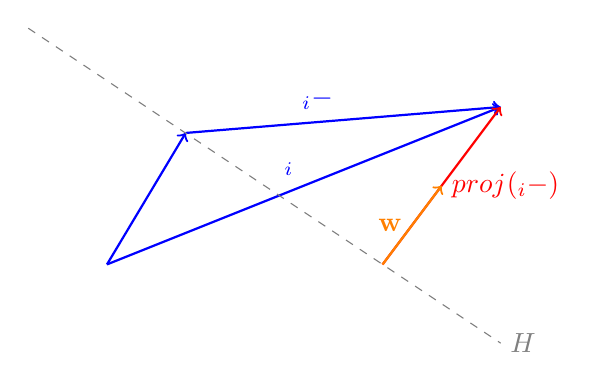
\begin{tikzpicture}
    % Define coordinates
    \coordinate (x) at (0,0);
    \coordinate (xi) at (3,2);
    \coordinate (w) at (1,-1);

    % Draw vector x
    \draw[->, thick, blue] (0,0) -- (1,1.67) node[midway, above left] {$\x$};
    \draw[->, thick, blue] (0,0) -- (5,2) node[midway, above left] {$\x_i$};
    \draw[->, thick, blue] (1,1.67) -- (5,2) node[midway, above left] {$\x_i-\x$};

      % Draw hyperplane
    \draw[dashed, gray] (-1,3) -- (5,-1) node[right] {$H$};

      % Draw projection
    \draw[->, thick, red] (3.5,0) -- (5,2) node[midway, right] {$\text{proj}_{\w}(\x_i - \x)$};

      % Draw vector w
    \draw[->, thick, orange] (3.5,0) -- (4.25,1) node[midway, left] {$\mathbf{w}$};
  \end{tikzpicture}
\end{center}
Simplfiying, we can express this as
\begin{align*}
  \frac{\ip{\x_i-\x}{\w}}{\norm{\w}_2}
   & = \frac{\ip{\x_i}{\w} - \ip{\x}{\w}}{\norm{\w}_2} \tag{linearity}                \\
   & = \frac{\ip{\x_i}{\w} + b}{\norm{\w}_2} \tag{$\x \in H \Harr \ip{\x}{\w}+b = 0$} \\
   & = \frac{\y_i\hat y_i}{\norm{\w}_2}
\end{align*}
We now have something to maximize.
\begin{defn}[margin]
  Given a hyperplane $H := \{\x : \ip{\x}{\w} + b = 0\}$ separating the data,
  the \term{margin} is the smallest distance between a data point $\x_i$ and $H$.

  That is, $\min_i \frac{\y_i \hat y_i}{\norm{\w}_2}$.
\end{defn}
The goal is the maximize the margin across all possible hyperplanes:
\[ \max_{\w,b} \min_i \frac{\y_i \hat y_i}{\norm{\w}_2} \qq{s.t.} \forall i, \y_i \hat y_i > 0 \qq{where} \hat y_i := \ip{\x_i}{\w} + b \]
We claim that we can arbitrarily scale the numerator.
Let $c>0$.
Then, $(\w,b)$ has the same loss as $(c\w,cb)$ because
$\frac{\ip{\x_i}{c\w}+cb}{\norm{c\w}_2}
  = \frac{c\ip{\x_i}{\w}+cb}{c\norm{\w}_2}
  = \frac{\ip{\x_i}{\w}+b}{\norm{\w}_2}$.

Therefore, we can equivalently write
\[ \max_{\w,b} \frac{1}{\norm{\w}_2} \qq{s.t.} \min_i \y_i \hat y_i = 1 \qq{where} \hat y_i := \ip{\x_i}{\w} + b \]
or even better:
\[ \min_{\w,b} \norm{\w}_2^2 \qq{s.t.} \forall i,\y_i(\ip{\x_i}{\w} + b) \geq 1 \]

Finally, consider the points that are closest to the boundary.
\begin{defn*}
  For the separating hyperplane $H = \{\ip{\x_i}{\w}+b = 0\}$,
  the two \term{supporting hyperplanes} are the parallel hyperplanes
  $H_+ := \{\ip{\x_i}{\w}+b = 1\}$ and $H_- := \{\ip{\x_i}{\w}+b = -1\}$
  which represent the margin boundaries.

  A \term{support vector} is a data point $\x_i \in H_+ \cup H_-$.
\end{defn*}
The support vectors are rare, but decisive because they reach the boundary of the constraint.

\paragraph{Explanation from the dual perspective}
Recall the SVM quadratic program
\[ \min_{\w_b} \frac12\norm{\w}^2_2 \qq{s.t.} \forall i,\y_i(\ip{\x_i}{\w}+b) \geq 1 \]
Introduce Lagrangian multipliers (dual variables) $\symbf{\alpha} \in \R^n$.
\begin{align*}
    & \min_{\w,b}\max_{\symbf\alpha>\0} \frac12\norm{\w}^2_2 - \sum_i \alpha_i[\y_i(\ip{\x_i}{\w}+b)-1]                                          \\
  = & \min_{\w,b} \begin{cases}
                    +\infty              & \exists i,\y_i(\ip{\x_i}{\w}+b)<1 (\text{set $\alpha_i$ as $+\infty$})   \\
                    \frac12\norm{\w}_2^2 & \forall i,\y_i(\ip{\x_i}{\w}+b)\geq 1 (\text{set all $\alpha_i$ as $0$})
                  \end{cases} \\
  = & \min_{\w_b} \frac12\norm{\w}^2_2 \qc{s.t.} \forall i,\y_i(\ip{\x_i}{\w}+b) \geq 1
\end{align*}
Therefore, we only need to study the minimax problem.
Assuming that the problem is convex (which it is, outside the scope of the course),
we can express this as
\[
  \max_{\symbf\alpha>\0} \overbrace{\min_{\w,b} \underbrace{\frac12\norm{\w}^2_2 - \sum_i \alpha_i[\y_i(\ip{\x_i}{\w}+b)-1]}_{\Loss(\w,b,\alpha)}}^{\Loss(\alpha)}
\]
and take the derivative of the interior with respect to $\w$ and $b$:
\begin{align*}
  \pdv{\Loss(\w,b,\alpha)}{\w} & = \w - \sum_i \alpha_i \y_i \x_i = 0 \\
  \w^*                         & = \sum_i \alpha_i \y_i \x_i          \\
  \pdv{\Loss(\w,b,\alpha)}{b}  & = - \sum_i \alpha_i \y_i = 0         \\
  \sum_i \alpha_i \y_i         & = 0
\end{align*}
Substitute back into $\Loss(\alpha)$:
\begin{align*}
  \Loss(\alpha)
   & := \min_{\w,b} \frac12\norm{\w}^2_2 - \sum_i \alpha[\y_i(\ip{\x}{\w}+b)-1]                                                                                    \\
   & = \min_{\w,b} \frac12\norm{\w}^2_2 - \ip{\sum_i\alpha_i\y_i\x_i}{\w} - b\sum_i \alpha_i\y_i + \sum_i \alpha_i                                                 \\
   & = \frac12\norm{\sum_i \alpha_i \y_i \x_i}^2_2 - \ip{\sum_i\alpha_i\y_i\x_i}{\sum_i \alpha_i \y_i \x_i} + \sum_i \alpha_i \tag{s.t. $\sum_i \alpha_i\y_i = 0$} \\
   & = -\frac12\norm{\sum_i \alpha_i \y_i \x_i}^2_2 + \sum_i \alpha_i                                                         \tag{s.t. $\sum_i \alpha_i\y_i = 0$}
\end{align*}
Therefore, we can write the dual problem as
\[ \min_{\symbf\alpha\geq0} {-\sum_i \alpha_i} + \frac12 \sum_i\sum_j \alpha_i\alpha_j\y_i\y_j\ip{\x_i}{\x_j} \qq{s.t.} \sum_i \alpha_i\y_i = 0 \]
We prefer this dual problem because it admits a very easy way to
use a non-linear mapping $\x \xto{\phi} \phi(\x)$
to transform non-linearly separable data $\x$
into linearly separable $\phi(\x)$.
After applying the unknown non-linear mapping, we get
\[ \min_{\symbf\alpha\geq0} {-\sum_i \alpha_i} + \frac12 \sum_i\sum_j \alpha_i\alpha_j\y_i\y_j\textcolor{blue}{\ip{\phi(\x_i)}{\phi(\x_j)}} \qq{s.t.} \sum_i \alpha_i\y_i = 0 \]
which we can find \emph{without explicitly applying $\phi$}
by using the ``kernel trick'' from \cref{ch:kernel},
writing the \textcolor{blue}{inner product} directly as a non-linear function.

\section{Soft-Margin SVM}
\lecture{Jan 30}

One of the drawbacks of the hard-margin SVM is that the data must be linearly separable.
That is, there must exist a non-zero margin between the data.

If we have a small number of outliers on the wrong side of the decision boundary,
we can instead just penalize it in the loss.
We do this by relaxing the constraint in hard-margin SVM
and including failures in the objective function.

\begin{defn}[hinge loss]
  Given label $\y \in \{-1,+1\}$ and score $\hat y := \ip{\x}{\w}+b$,
  let $\y\hat y$ be the confidence.

  Define $\ell_{\hinge} = (1-\y\hat y)^+ = \begin{cases}
      1-\y\hat y & \y\hat y < 1     \\
      0          & \text{otherwise}
    \end{cases}$
\end{defn}

In general, notate $x^+$ to mean $\max\{x,0\}$.

Now, we can formulate the soft-margin SVM as
\begin{equation}\label{eq:ssvm}
  \boxed{
    \min_{\w,b} \textcolor{blue}{\frac12\norm{\w}^2_2}
    + \textcolor{orange}{C} \cdot \textcolor{red}{\sum_i(1-\y_i\hat y_i)^+}
    \qq{s.t.} \hat y_i = \ip{\x_i}{\w}+b
  }
\end{equation}
(\textcolor{blue}{margin maximization}, \textcolor{orange}{regularization hyperparameter}, \textcolor{red}{error penalty}).
Notice that the hard-margin SVM is the limiting behaviour
of the soft-margin SVM as $C \to \infty$.

\paragraph{Why do we use the hinge loss?}
Consider the probability that $\Y \neq \sgn(\hat \Y)$
\begin{align*}
  \Pr[\Y \neq \sgn(\hat \Y)]
  = \Pr[\Y\hat\Y \leq 0]
  = \E[\I[\Y\hat\Y \leq 0]]
  =: \E[\ell_{0-1}(\Y\hat\Y)]
\end{align*}
We want to minimize $\E[\ell_{0-1}(\Y\hat\Y)]$.
Minimizing this value is hard because $\ell_{0-1}$ is discontinuous at 0
and has gradient $\vb 0$ almost everywhere.

By Bayes' rule, we can rewrite as
$\E_{\vv X}\E_{\Y \mid \vv X}[\ell_{0-1}(\Y\hat\Y)]$.
Then, we can minimize instead
\[ \eta(\x) = \argmin_{\hat y \in \R} \E_{\Y \mid \vv X=\x}[\ell_{0-1}(\Y\hat y)] \]
since setting $\Y = \eta(\vv X)$.

\begin{defn}[classification calibrated]
  We say a loss function $\ell(\y\hat y)$ is \term{classification calibrated}
  if for all $\x$,
  \[ \hat\y(\x) := \argmin_{\hat y \in \R}\E_{\Y \mid \vv \X=\x}[\ell(Y\hat y)] \]
  has the same sign as the Bayes rule $\eta(\x)$.
\end{defn}

Due to Bartlett, we have a helpful theorem
\begin{theorem}[characterization under convexity]
  Any convex loss $\ell$ is classification calibrated if and only if
  $\ell$ is differentiable at 0 and $\ell'(0) < 0$.
\end{theorem}
\begin{corollary}
  A classifier that minimizes the expected hinge loss
  also minimizes the expected 0-1 loss.
\end{corollary}

This theorem is also one of the big reasons why the perceptron
cannot generalize well.

\begin{remark}
  The perceptron loss $\ell(\y\hat y) = -\min\{\y\hat y,0\}$
  is not differentiable at 0,
  so it is not classification calibrated and cannot generalize.
\end{remark}

\paragraph{Generating the dual}
Recall the soft-margin SVM
\[
  \min_{\w,b} \frac12\norm{\w}^2_2
  + C\cdot \sum_i(1-\y_i(\ip{\x_i}{\w}+b))^+
\]
Notice that we can write
$C\cdot(t)^+ = \max\{Ct,0\} = \max_{0 \leq \alpha \leq C} \alpha t$
to get
\[
  \min_{\w,b} \max_{0 \leq \symbf{\alpha} \leq C}
  \frac12\norm{\w}^2_2
  + \sum_i\alpha_i(1-\y_i(\ip{\x_i}{\w}+b))
\]
As before, swap min with max:
\[
  \max_{0 \leq \symbf{\alpha} \leq C} \overbrace{
    \min_{\w,b} \underbrace{
      \frac12\norm{\w}^2_2 + \sum_i\alpha_i(1-\y_i(\ip{\x_i}{\w}+b))
    }_{\Loss(\w,b,\alpha)}
  }^{\Loss(\alpha)}
\]
Now, set our optimality conditions
\begin{align*}
  \pdv{\Loss(\w,b,\alpha)}{\w} & = \w - \sum_i \alpha_i \y_i \x_i = \vb 0 &
  \pdv{\Loss(\w,b,\alpha)}{b}  & = -\sum_i \alpha_i \y_i = 0                \\
  \w                           & = \sum_i \alpha_i \y_i \x_i              &
  \sum_i\alpha_i\y_i           & = 0
\end{align*}
and substitute into $\Loss(\alpha)$:
\begin{align*}
  \Loss(\alpha)
   & := \frac12\norm{\w}^2_2 + \sum_i\alpha_i(1-\y_i(\ip{\x_i}{\w}+b))                              \\
   & = \frac12\norm{\sum_i \alpha_i \y_i \x_i}^2_2 + \sum_i\alpha_i - \ip{\sum_i \alpha_i \y_i\x_i} \\
   & = -\frac12\norm{\sum_i \alpha_i \y_i \x_i}^2_2 + \sum_i \alpha_i
\end{align*}
Switching from max to min and expanding the norm, we get
\begin{equation}\label{eq:ssvmd}
  \boxed{
    \min_{0 \leq \symbf{\alpha} \leq C}
    -\sum_i \alpha_i +
    \frac12 \sum_i \sum_j \alpha_i \alpha_j y_i y_j \ip{\x_i}{\x_j}
    \qq{s.t.}
    \sum_i \alpha_i \y_i = 0
  }
\end{equation}
which is identical to the hard-margin SVM dual with an upper bound $C$ on $\symbf\alpha$.

\lecture{Feb 1}

Suppose we solve the dual (\cref{eq:ssvmd}) with optimal solution $\symbf\alpha^*$.
Then,
\begin{equation}\label{eq:ssvmw}
  \w^* = \sum \alpha^*_i \y_i \x_i.
\end{equation}
If we have a point on $H_{\pm 1}$, i.e., $\y\hat y = 1$,
we can recover $b^*$ as $\y - \ip{\x}{\w^*}$.

\paragraph{Training by gradient descent}
Suppose we have a minimization problem $\min_{\x} f(\x)$.
Then, to make a guess $\x$ better, set $\x \gets \x - \eta \cdot \nabla_{\x} f(\x)$
for some \term{learning rate} $\eta > 0$.

Given the problem
\[
  \min_{\w,b} \frac{1}{2\lambda} \norm{\w}_2^2 + \frac1n \sum_i \ell(\y_i\hat y_i)
  \qq{where}
  \hat y_i = \ip{\x_i,\w} + b
\]
with loss function $\ell$, the gradient descent steps are
\begin{align*}
  \w & \gets \w - \eta \cdot \nabla_{\w}\qty(\frac{1}{2\lambda} \norm{\w}_2^2 + \frac1n \sum_i \ell(\y_i\hat y_i)) \\
     & = \w - \eta \qty[\frac{\w}{\lambda} + \frac1n \sum_i \ell'(\y_i\hat y_i)\y_i\x_i]                           \\
  b  & \gets b - \eta \cdot \nabla_b\qty(\frac{1}{2\lambda} \norm{\w}_2^2 + \frac1n \sum_i \ell(\y_i\hat y_i))     \\
     & = b - \eta \qty[\frac1n\sum_i \ell'(\y_i \hat y_i)\y_i]
\end{align*}
because $\nabla_{\w} \ell(\y_i\hat y_i) = \ell'(\y_i\hat y_i)\cdot\y_i\nabla_{\w}(\hat y_i) = \ell'(\y_i\hat y_i)\y_i\x_i$
and $\nabla_b \ell(\y_i\hat y_i) = \ell'(\y_i\hat y_i)\cdot\y_i \nabla_b(\hat y_i) = \ell'(\y_i\hat y_i)\cdot \y_i$.

\section{Reproducing Kernels}\label{ch:kernel}
\newcommand{\phix}[1]{\mqty[\vec{#1#1\trans} \\ \sqrt{2}#1 \\ 1]}

We have dealt with data that is perfectly linearly separable (hard-margin SVM)
and mostly linearly separable (soft-margin SVM).

\begin{problem}
  How can we use our existing techniques to classify
  a fully non-linearly separable dataset?
\end{problem}

In the linear classifier, we used an affine function $\ip{\w}{\x}+b$.
Now, we define a quadratic classifier.

\begin{defn}[quadratic classifier]
  A function $f : \R^d \to \R^d$ of the form $f(\x) = \ip{\x}{Q\x} + \sqrt{2}\ip{\x}{\p} + b$
  where the weights to be learned are $Q \in \R^{d\times d}$, $\p \in \R^d$, and $b \in \R$.
\end{defn}

Recall from linear algebra that for all $A$, $B$, $C$, $\ip{AB}{C} = \ip{B}{A\trans C}$
and $\ip{A}{BC} = \ip{AB\trans}{C}$.

\begin{defn}[matrix vectorization]
  Given a matrix $\vb{A} \in \R^{m\times n}$,
  let $\vec{\vb{A}} \in \R^{mn}$ be its vectorization.
  That is,
  \[
    \vb A = \mqty[a_{11} & a_{12} & \cdots & a_{1n} \\ a_{21} & a_{22} & \cdots & a_{2n} \\ \vdots & \vdots & \ddots & \vdots \\ a_{m1} & a_{m2} & \cdots & a_{mn}]
    \implies
    \vec{\vb A} = \mqty[a_{11} \\ a_{12} \\ \vdots \\ a_{1n} \\ \vdots \\ a_{mn}]
  \]
\end{defn}

Then, we can write the quadratic classifier as:
\begin{align*}
  f(\x) & =  \ip{\x}{Q\x} + \sqrt{2}\ip{\x}{\p} + b       \\
        & =  \ip{\x\x\trans}{Q} + \ip{\sqrt{2}\x}{\p} + b \\
        & = \ip{\phix{\x}}{\bmqty{\vec{Q}                 \\\p\\b}}
\end{align*}
If we write $\phi(\x) = (\vec{\x\x\trans}, \sqrt{2}\x, 1)\trans$
and $\w = (\vec{Q}, \p, b)\trans$,
then we can write $f$ as
\[ f(\x) = \ip{\phi(\x)}{\w} \]
but this really blows up the dimension to $\R^{d^2+d+1}$.
Recall that in the dual forms of SVM,
all we need is to know the inner product $\ip{\phi(\x)}{\phi(\w)}$.
With our new $\phi$, we get
\begin{align*}
  k(\x,\z) := \ip{\phi(\x)}{\phi(\z)}
   & = \ip{\phix{\x}}{\phix{\z}}                                             \\
   & = \ip{\vec{\x\x\trans}}{\vec{\z\z\trans}} + \ip{\sqrt2\x}{\sqrt2\z} + 1 \\
   & = \ip{\x}{\z}^2 + 2\ip{\x}{\z} + 1                                      \\
   & = (\ip{\x}{\z} + 1)^2
\end{align*}

This process is easily reproducable for a given $\phi$.
What about the other direction?

\begin{defn}[reproducing kernel]
  We call $k : \mathcal{X} \times \mathcal{X} \to \R$
  a \term{reproducing kernel} if there exists some $\phi : \mathcal{X} \to \mathcal{H}$
  so that $\ip{\phi(\x)}{\phi(\z)} = k(\x,\z)$.
\end{defn}

\begin{remark}
  When such a kernel exists, it may not be unique.

  For example, the kernels $\phi(\x) = [x_1^2,\sqrt2 x_1x_2,x_2^2] \in \R^3$
  and $\psi(\x) = [x_1^2,x_1x_2,x_1x_2,x_2^2] \in \R^4$
  have the same inner product $\ip{\phi(\x)}{\phi(\z)} = \ip{\psi(\x)}{\psi(\z)}$.
\end{remark}

\begin{theorem}[Mercer's theorem]
  $k : \mathcal{X} \times \mathcal{X} \to \R$ is a kernel if and only if
  for any $n \in \N$ and any $\x_1,\dotsc,\x_n \in \mathcal{X}$,
  the \term{kernel matrix} $K_{ij} := k(\x_i,\x_j)$ is symmetric and positive semi-definite.
\end{theorem}

Recall from linear algebra: $K$ is \term{symmetric} if $K_{ij} = K_{ji}$ for all indices,
and \term{positive semi-definite} if $\ip{\symbf\alpha}{K\symbf\alpha} \geq 0$ for all vectors $\symbf\alpha$.

The proof is extremely convoluted and well beyond the scope of the course.

\begin{example}
  The following are kernels:
  \begin{itemize}
    \item the polynomial kernel $k(\x,\z) = (\ip{\x}{\z} + 1)^p$ for hyperparameter $p$,
    \item the Gaussian kernel $k(\x,\z) = \exp(-\norm{\x-\z}_2^2/\sigma)$ for hyperparameter $\sigma$, and
    \item the Laplace kernel $k(\x,\z) = \exp(-\norm{\x-\z}_2/\sigma)$ for hyperparameter $\sigma$
  \end{itemize}
\end{example}

Now, we can substitute our expression for the inner product to \cref{eq:ssvm,eq:ssvmd},
the primal and dual of the soft-margin SVM:
\begin{gather*}
  \min_{\w,b} \frac12\norm{\w}_2^2 + C\cdot\sum_i(1-\y_i\hat y_i)^+
  \qq{s.t.} \hat y_i = \ip{\phi(\x_i)}{\w} \\
  \min_{0 \leq \symbf{\alpha} \leq C}
  -\sum_i \alpha_i + \frac12 \sum_i \sum_j \alpha_i \alpha_j y_i y_j k(\x_i,\x_j)
  \qq{s.t.} \sum_i \alpha_i \y_i = 0
\end{gather*}

Once we solve $\symbf\alpha^*$, we can try to recover $\w^*$ as in \cref{eq:ssvmw}
\[ \w^* = \sum \alpha_i^*\y_i \phi(\x_i) \]
but this will not work since we do not know $\phi$ explicitly.
Instead, we only need to compute the score function
\begin{align*}
  f(\x) & := \ip{\phi(\x)}{\w^*}                          \\
        & = \ip{\phi(\x)}{\sum \alpha_i^*\y_i \phi(\x_i)} \\
        & = \sum \alpha_i^*\y_i \ip{\phi(\x)}{\phi(\x_i)} \\
        & = \sum \alpha_i^*\y_i k(\x,\x_i)
\end{align*}
and return $\sgn(f(\x))$.

\section{Gradient Descent}\label{ch:gd}

% \chapter{Neural Networks}

% \chapter{Modern Machine Learning}

% \chapter{Trustworthy Machine Learning}

\end{document}
